% Created 2023-10-30 Mon 17:35
% Intended LaTeX compiler: pdflatex
\documentclass[presentation,smaller]{beamer}
\usepackage[utf8]{inputenc}
\usepackage[T1]{fontenc}
\usepackage{graphicx}
\usepackage{longtable}
\usepackage{wrapfig}
\usepackage{rotating}
\usepackage[normalem]{ulem}
\usepackage{amsmath}
\usepackage{amssymb}
\usepackage{capt-of}
\usepackage{hyperref}
\usepackage[most]{tcolorbox}
\newtcbox{\badge}[1][red]{on line, arc=2pt, colback=#1!50!black, colframe=#1!50!black, fontupper=\color{white}, boxrule=1pt, boxsep=0pt, left=6pt, right=6pt, top=2pt, bottom=2pt}
\usepackage{subcaption}
\captionsetup{labelformat=empty}
\captionsetup[subfigure]{labelformat=empty}
\usetheme{MIS}
\author{vopuu}
\date{\today}
\title{}
\begin{document}


\section*{Introduction}
\label{sec:orgf60894a}

\begin{frame}[label={sec:org1a25345}]{Protein Design}
\begin{center}
\Large\textbf{Engineer proteins for desirable properties}
\end{center}
\end{frame}

\begin{frame}[label={sec:org876a0c1}]{Experimental Approaches}
\begin{itemize}
\item Techniques such as directed evolution, phage display, and yeast display.
\item Iterative process of mutation and selection in directed evolution.
\item Structural validation using X-ray crystallography and cryo-EM.
\item Notable successes include enhanced green fluorescent protein (eGFP) and evolved enzymes.
\end{itemize}

\begin{center}
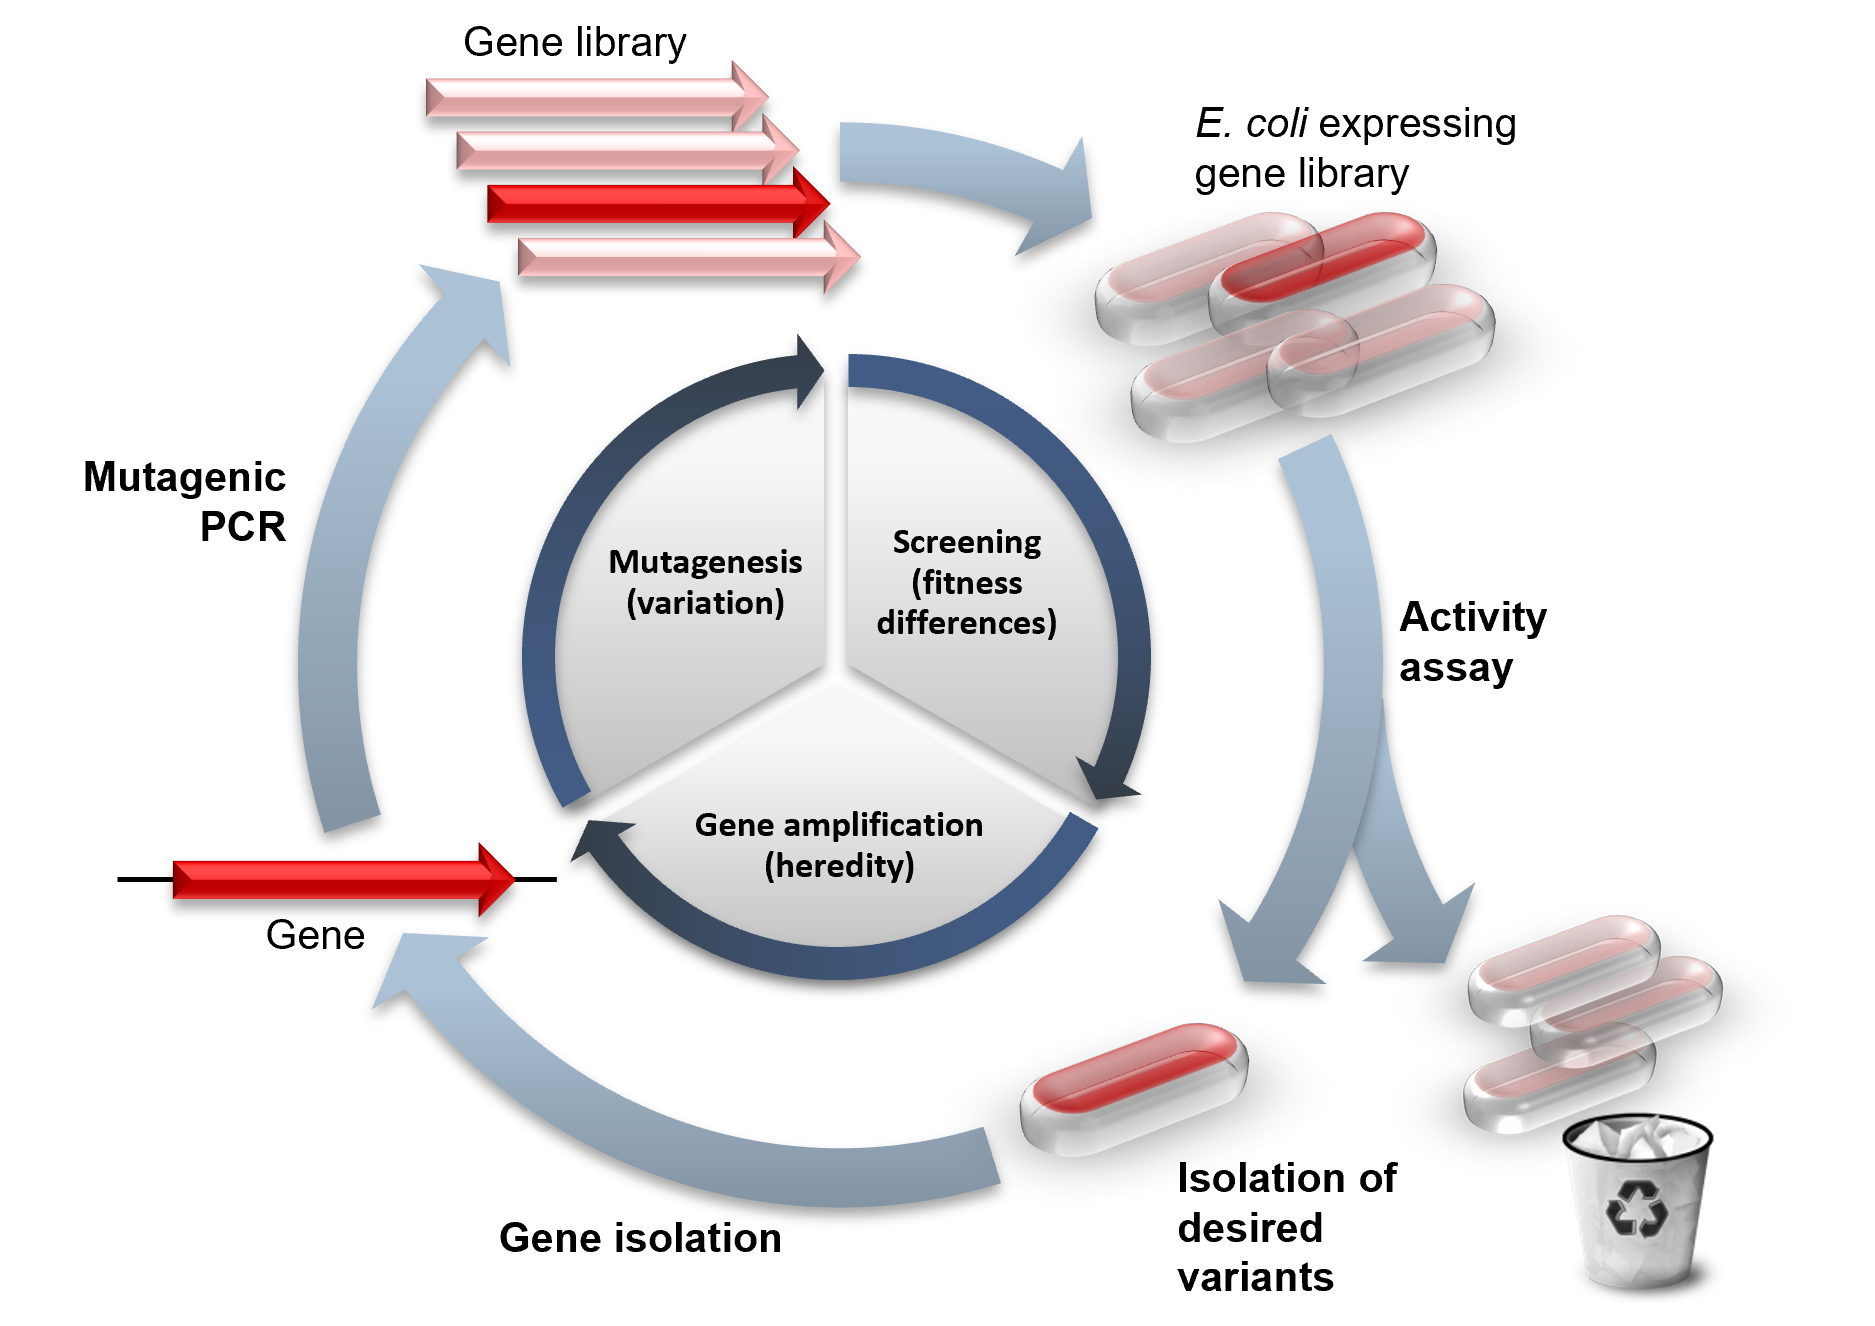
\includegraphics[width=0.5\textwidth]{./img/DE_cycle.png}
\end{center}
(credits wiki directed evolution)
\end{frame}
\begin{frame}[label={sec:orgfa49bf7}]{Computational Protein Design}
\begin{itemize}
\item Tools like Rosetta and FoldX for structure prediction and design.
\item Enables rapid exploration of vast sequence and conformational spaces.
\item Design of novel enzymes, e.g., Kemp eliminase.
\item Creation of protein switches and custom therapeutics.
\end{itemize}
\end{frame}

\begin{frame}[label={sec:orgd7412f5}]{Why Computational Design is Desirable}
\begin{itemize}
\item \alert{\alert{Speed}}: Computational methods can quickly scan vast design spaces.
\begin{itemize}
\item 100 amino acids proteins \(\implies\) \(20^{100} \approx 10^{91} \gt\) |atoms in
v. universe|
\end{itemize}
\item \alert{\alert{Precision}}: Allows for targeted design based on specific criteria.
\item \alert{\alert{Cost-Effective}}: Reduces the need for extensive lab work and resources.
\item \alert{\alert{Predictive Power}}: Can forecast how changes in sequence affect structure and function.
\item \alert{\alert{Synergy}}: Complements experimental methods by narrowing down candidates and guiding lab efforts.
\end{itemize}
\end{frame}


\begin{frame}[label={sec:org6b95476}]{The Problem: Physics-Based Approach}
\begin{block}{Definition}
\begin{itemize}
\item Predict 3D protein structures from sequences.
\end{itemize}
\end{block}

\begin{block}{Historical Insight}
\begin{itemize}
\item Structure dictates function.
\item Nature's "folds" reveal protein functions.
\end{itemize}
\end{block}

\begin{block}{Modern Bioinformatics Goal}
\begin{itemize}
\item Design sequences for desired 3D structures and functions.
\end{itemize}

\begin{center}
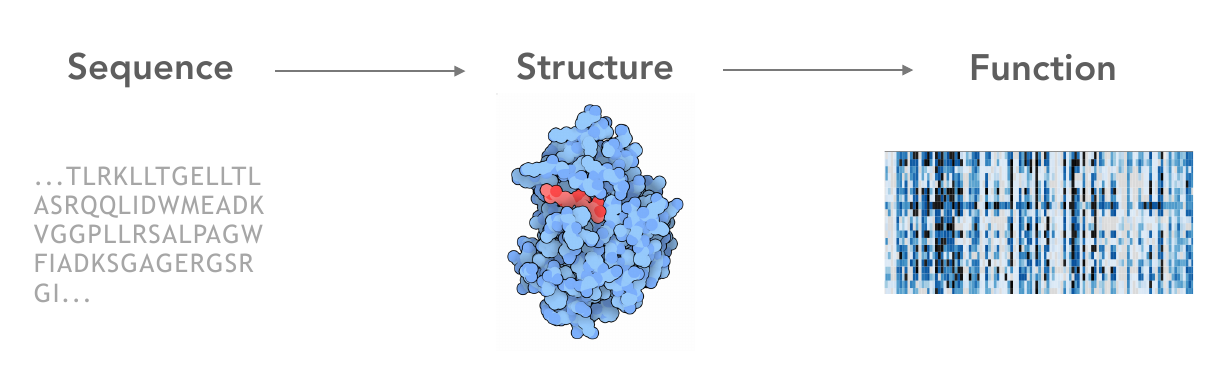
\includegraphics[width=.9\linewidth]{./img/s1_f1.png}
\end{center}
(credits E. Laine)
\end{block}
\end{frame}

\begin{frame}[label={sec:org4ef97f1}]{Protein Design Principles}
\begin{block}{The Core Challenge: Optimization}
Objective: Design protein sequences to achieve specific structures and functions.
\begin{block}{Starting Point: Known Structures}
Utilize established protein folds with recognized functions as templates.
\end{block}
\begin{block}{The Dual Nature of the Problem}
Traditional Folding: Given a sequence, predict its structure.
Inverse Folding (Design): For a desired structure, determine or design the optimal sequence.

\begin{center}
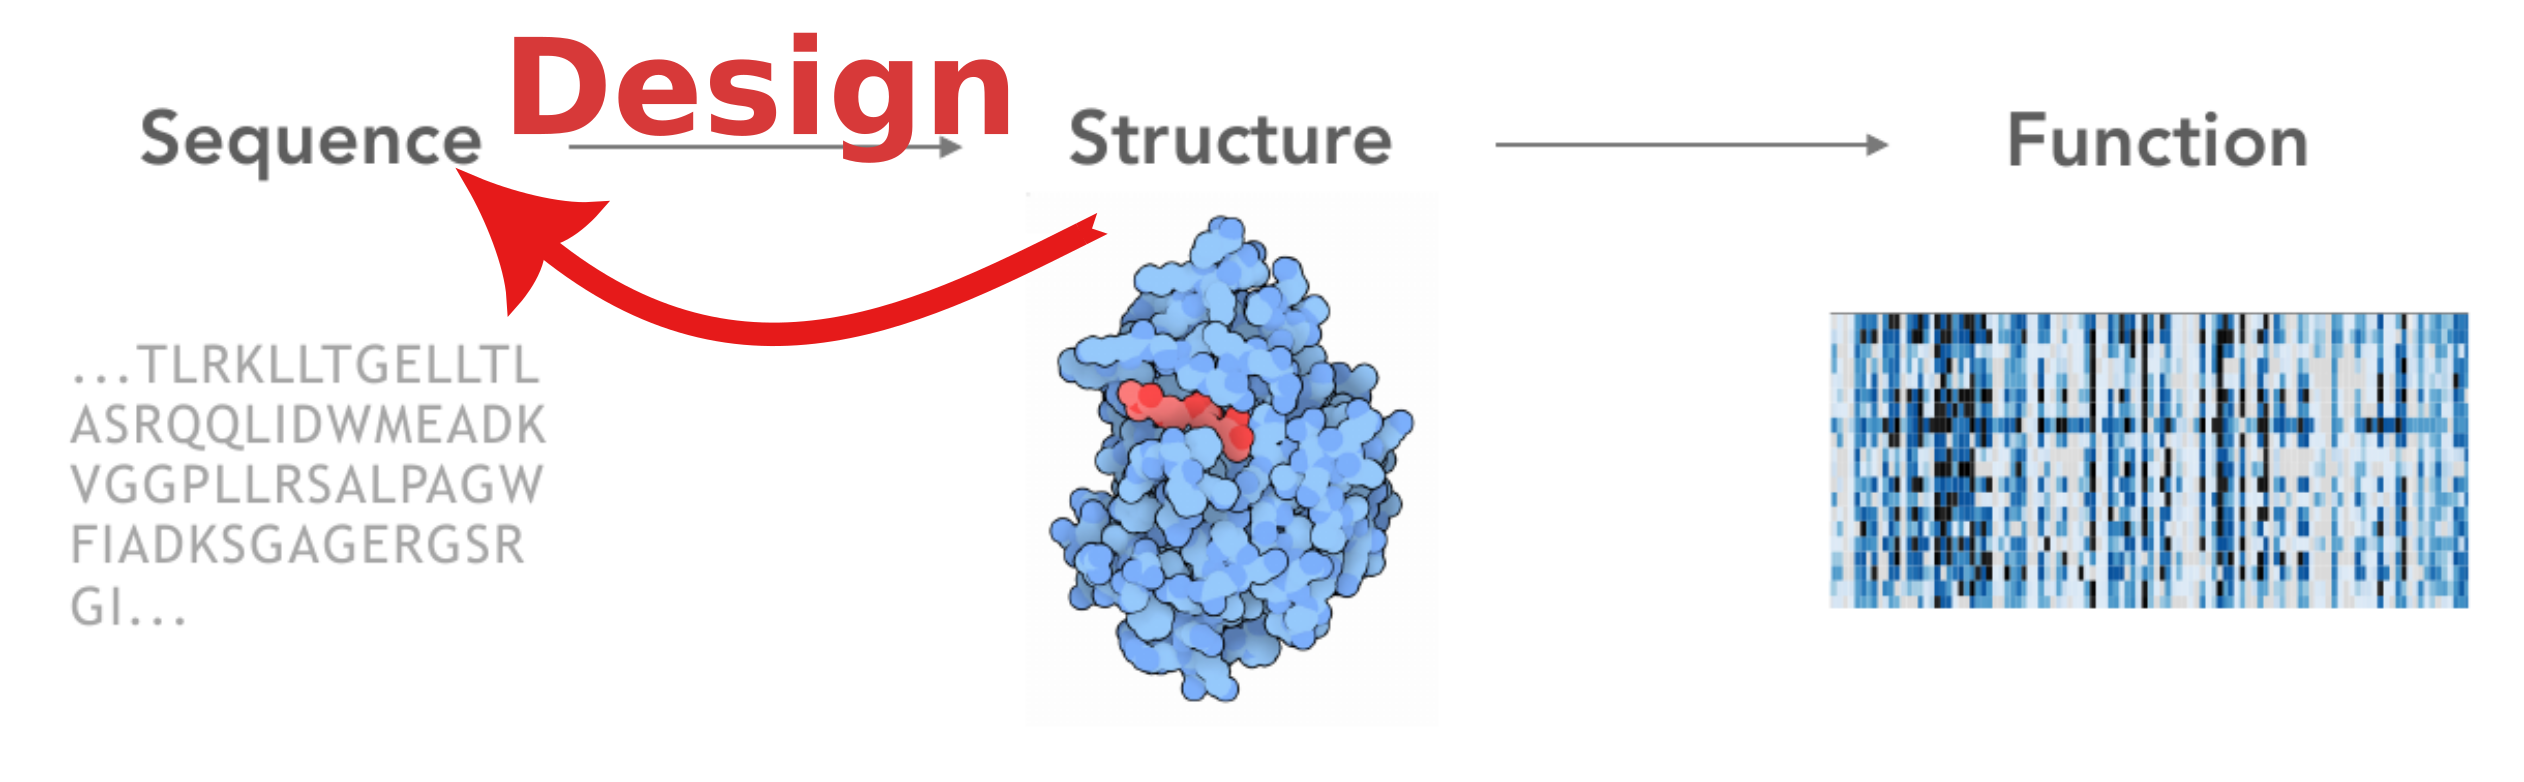
\includegraphics[width=.9\linewidth]{./img/s1_f2.png}
\end{center}
(credits E. Laine)
\end{block}
\end{block}
\end{frame}

\begin{frame}[label={sec:orgef5e774}]{Design = inverse protein design}
\begin{columns}
\begin{column}{0.5\columnwidth}
\begin{block}{The Essence of Folding: Free Energy}
Protein folding is driven by changes in free energy.
Equation: \(\Delta\) G = \(\Delta\) H - T \(\Delta\) S
\end{block}

\begin{block}{Visualizing the Folding Process}
Proteins transition from a less ordered (unfolded) state to a highly ordered
(folded) structure. Representation: "Unfolded → Folded"
\end{block}
\end{column}

\begin{column}{0.5\columnwidth}
\begin{center}
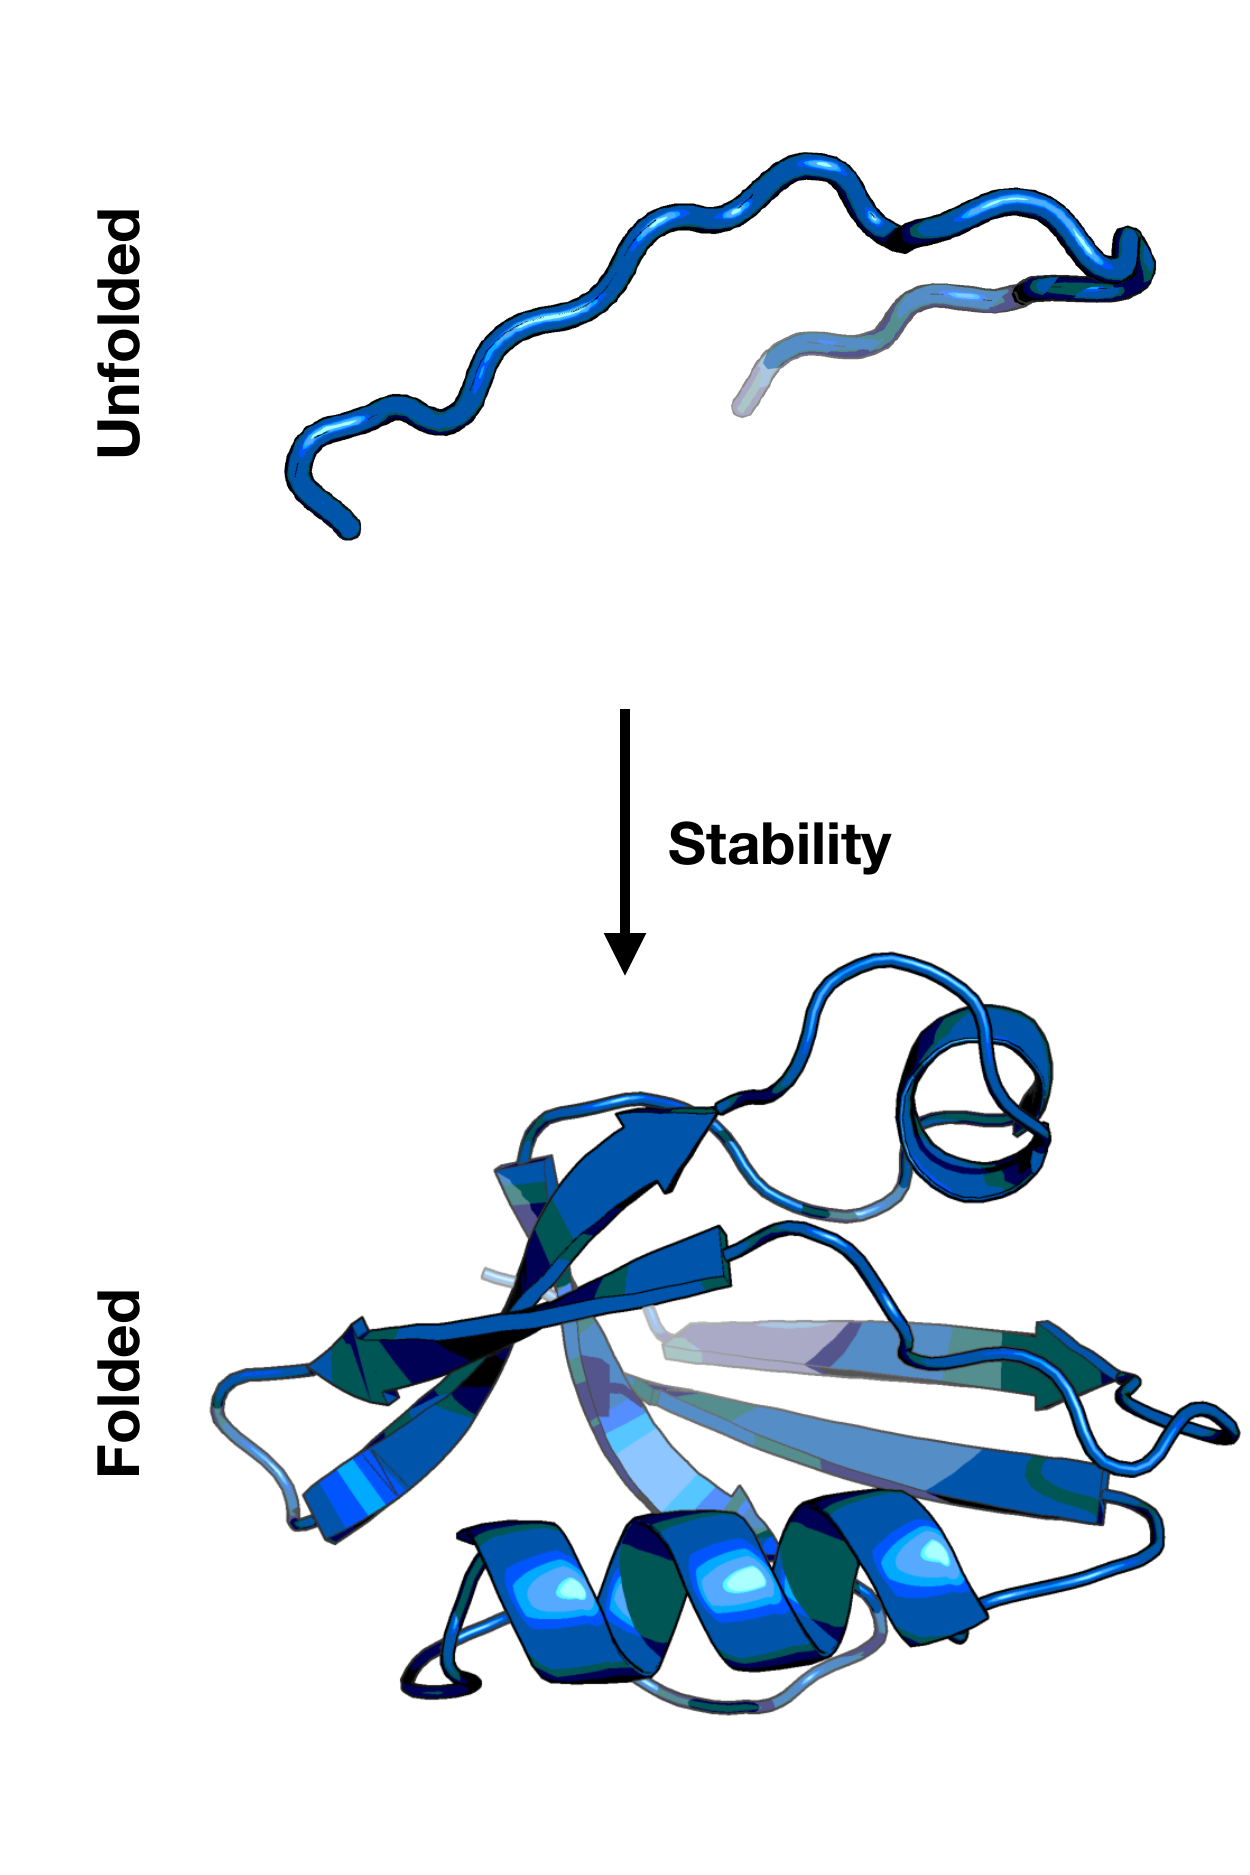
\includegraphics[width=0.7\textwidth]{./img/s1_f3.png}
\end{center}
\end{column}
\end{columns}
\end{frame}

\begin{frame}[label={sec:orgfa85518}]{Usually not realistic}
\begin{center}
\includegraphics[width=.9\linewidth]{./img/s1_f4.png}
\end{center}

(credits Pr. F. Noe, F. U. Berlin)
\end{frame}

\begin{frame}[label={sec:org858a799}]{Usual timescale for the folding process}
\begin{center}
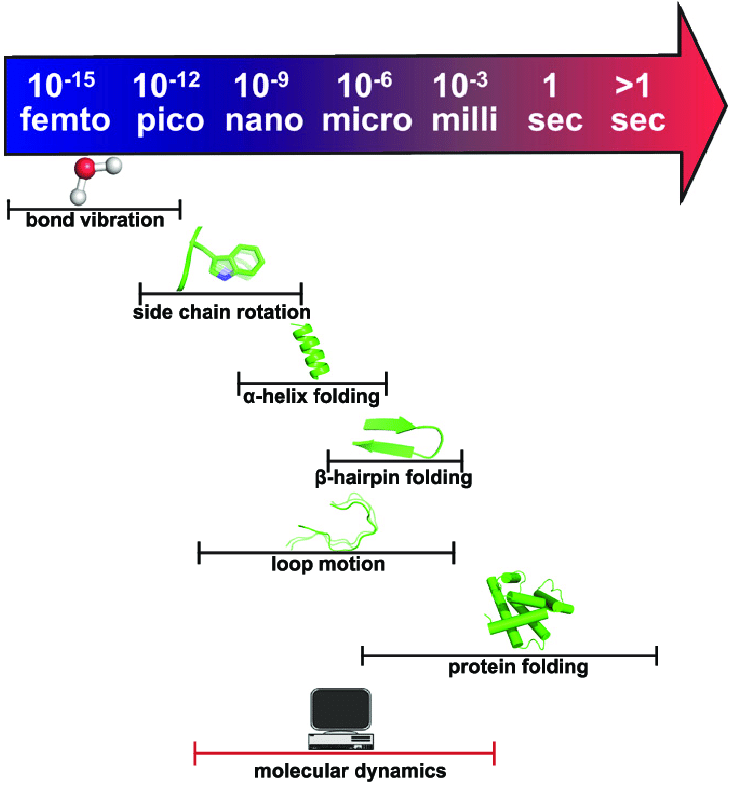
\includegraphics[width=0.6\textwidth]{./img/time_scale.png}
\end{center}

Interesting phenomena take time
(credits Werner, Tim, et al. Advanced drug delivery reviews (2012))
\end{frame}

\begin{frame}[label={sec:org4cee387}]{Exploring Protein Conformations}
\begin{block}{The Challenge of Flexibility}
\begin{columns}
\begin{column}{0.6\columnwidth}
Proteins are inherently flexible, leading to a vast conformational space.
Combinatorial explosion example:
For a rotation (θ) of 30°:
\begin{itemize}
\item N=2: 144 conformations
\item N=3: 21,000 conformations
\item N=5: 430,000,000 conformations
\end{itemize}
\end{column}

\begin{column}{0.4\columnwidth}
\begin{center}
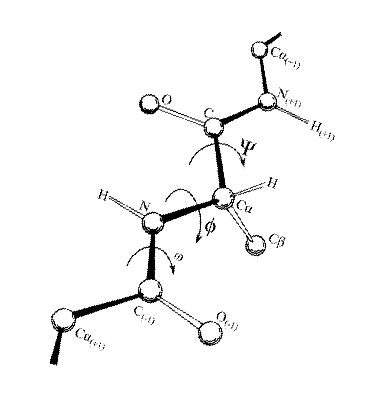
\includegraphics[width=0.5\textwidth]{./img/s1_f5.png}
\end{center}
\end{column}
\end{columns}
\end{block}

\begin{block}{Simplifying with Approximations}
Fixed Backbone: Retain the protein's main structure, only vary side chains. Use
of rotamer libraries: Discretized conformations for amino acid side chains.
\end{block}

\begin{block}{Modeling the Unfolded State}
\begin{itemize}
\item Primary approach: The solvated short peptide model.
\item Alternative: Statistical models derived from observational data.
\end{itemize}
\end{block}
\end{frame}

\begin{frame}[label={sec:org8e2f174}]{Navigating the Protein Sequence Space}
\begin{block}{Probabilistic Approaches}
Delve into the vast sequence space using stochastic methods.
\begin{itemize}
\item Markov Chain Monte Carlo (MCMC): A random sampling method to explore possible
sequences.
\item Genetic Algorithm: Mimics natural selection to optimize sequences.
\end{itemize}
\end{block}
\begin{block}{Deterministic Search for Optimal Conformations}
\begin{itemize}
\item Aim: Identify the sequence with the lowest possible energy.
\item Dead End Elimination (DEE): Systematically eliminates unlikely sequences to
pinpoint the Global Minimum Energy Conformation (GMEC).
\end{itemize}
\end{block}
\end{frame}

\begin{frame}[label={sec:org78512e5}]{Understanding the Unfolded State}
\begin{block}{Modeling Exposed Residues}
\begin{itemize}
\item In the unfolded state, residues are fully exposed \(\implies\) no interactions.
\item Energy Model:
\begin{itemize}
\item \(E^{uf}(S) = \sum_{i} E^{uf}(S_i)\)
\item Calculates the energy based on individual amino acids.
\end{itemize}
\end{itemize}
\end{block}

\begin{block}{Refining the Model}
\begin{itemize}
\item Parameterization for accuracy.
\begin{itemize}
\item Use experimental data and computational methods.
\end{itemize}
\end{itemize}
\end{block}
\end{frame}

\section*{Computational protein design: for the fold}
\label{sec:org58cda33}

\begin{frame}[label={sec:orgee4897f}]{Test case: redesigning the PDZ fold}
\begin{block}{The target fold: PDZ}
\begin{itemize}
\item PDZ domains are protein structural domains that are often found in signaling
proteins. They play a role in anchoring receptor proteins in the membrane and
recruiting specific proteins to specific sites in the cell.
\end{itemize}
\end{block}
\begin{block}{What it does?}
\begin{itemize}
\item PDZ domains typically bind to the C-terminus of other proteins, facilitating
protein-protein interactions.
\end{itemize}

\begin{center}
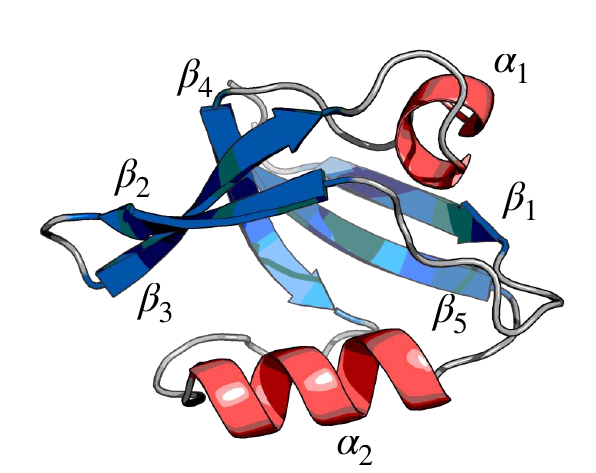
\includegraphics[width=0.5\textwidth]{./img/pdz_struct.png}
\end{center}
\end{block}
\end{frame}

\begin{frame}[label={sec:org8443889}]{Sampling sequences}
\begin{block}{The model}
\begin{itemize}
\item MM + Implicit model + Empirical unfolded model
\item 10\textsuperscript{8} MCMC steps
\end{itemize}
\begin{center}
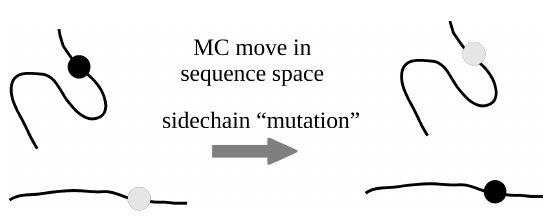
\includegraphics[width=0.5\textwidth]{./img/mcmc_move.png}
\end{center}
\end{block}

\begin{block}{MCMC sampling}
\begin{center}
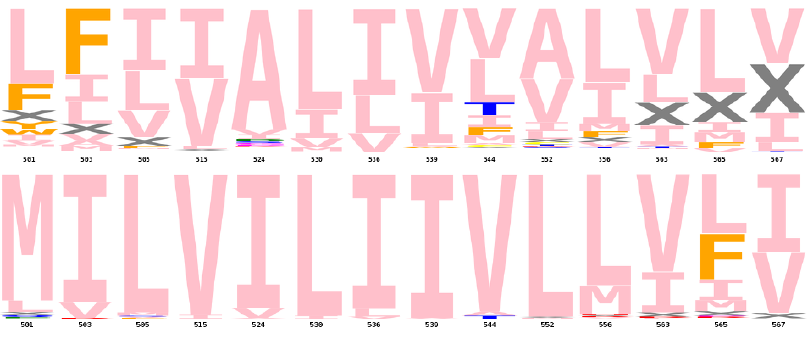
\includegraphics[width=0.6\textwidth]{./img/logo_design_pdz.png}
\end{center}
\end{block}
\end{frame}

\begin{frame}[label={sec:org3d33dd1}]{MD simulations}
You actually don't fold them as the folding is too expensive

\begin{center}
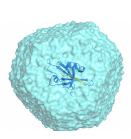
\includegraphics[width=0.3\textwidth]{./img/solvated_system.png}
\end{center}

For each selected sequence: 1) Solvate then 2) simulate for stability.
\begin{block}{MD settings}
\begin{itemize}
\item \(0.2 \mu s\) \(\leftrightarrow\) 2 weeks on 200 CPUs
\end{itemize}


(Opuu \emph{et al} (2020) Sci. Rep.)
\end{block}
\end{frame}

\begin{frame}[label={sec:orgb2d635a}]{Computational enzyme design}
\begin{center}
\Large\textbf{Design for the binding or catalysis}
\end{center}
\end{frame}

\begin{frame}[label={sec:org0007ddd}]{The problem definition}
\begin{columns}
\begin{column}{0.5\columnwidth}
\begin{block}{Definition of the problem}
Find a sequence that can bind a specific substrat | catalyze a specific reaction

Shift of paradigm!
\end{block}
\begin{block}{What for?}
Develop enzymes:
\begin{itemize}
\item that degrade plastic
\item that catalyze the synthesis of bio-fuel
\item that allow the incorporation of new chemistry in proteins
\end{itemize}
\end{block}
\end{column}
\begin{column}{0.5\columnwidth}
\begin{center}
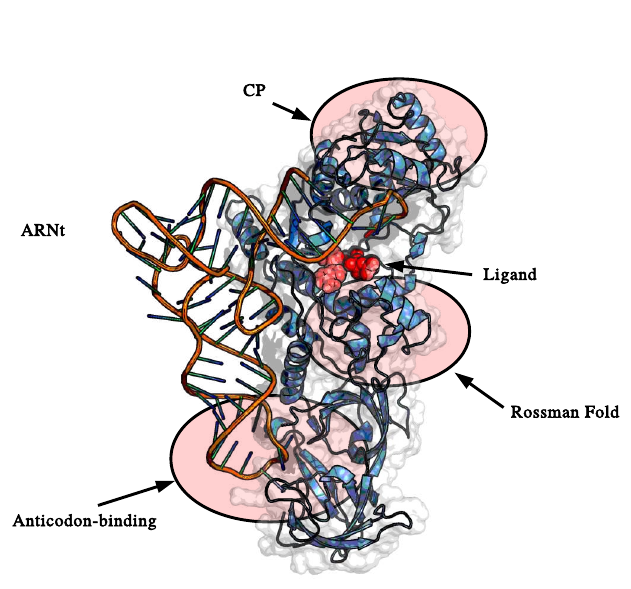
\includegraphics[width=.9\linewidth]{./img/enzyme_struct.png}
\end{center}
\end{column}
\end{columns}
\end{frame}

\begin{frame}[label={sec:org25e060b}]{The energy bottleneck}
\begin{block}{The reaction pathway}
\begin{itemize}
\item The series of molecular events during a reaction.
\end{itemize}

\begin{center}
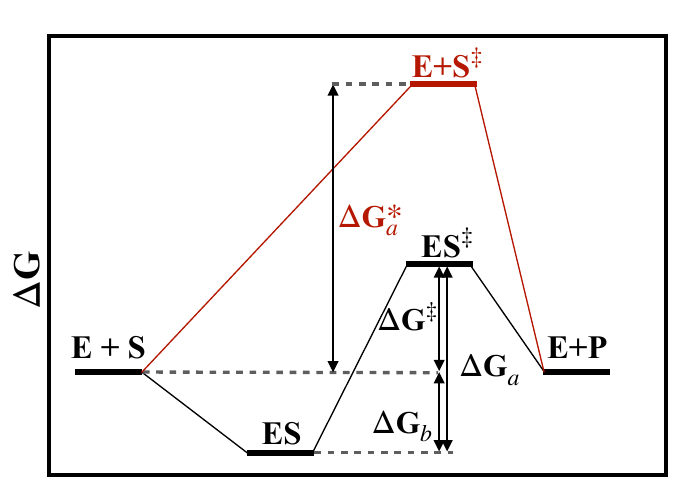
\includegraphics[width=0.5\textwidth]{./img/reaction_pathway.png}
\end{center}
\end{block}

\begin{block}{Define the optimization problem}
\begin{itemize}
\item Binder: find mutations that improve the binding \(\Delta G_{b}\)
\item Catalyzer: find mutations that improve the catalysis \(\Delta G^{\ddagger}\)
\end{itemize}
\end{block}
\end{frame}

\begin{frame}[label={sec:orgcd28d5a}]{Designing a strong binder}
\begin{columns}
\begin{column}{0.6\columnwidth}
\begin{block}{MetRS: binding unatural ligand}
\begin{itemize}
\item \(\Delta G(\text{Unbound} \rightarrow \text{Bound})\)
\end{itemize}
\end{block}

\begin{block}{Sampling technique}
\begin{itemize}
\item Adaptive landscape flattening:
\begin{itemize}
\item MCMC to create a surrogate model of the unbound state \(\Delta G_{u}\)
\item Combine with the bound state \(\rightarrow\) \(\Delta G_{b} - \Delta G_{u}\)
\end{itemize}
\end{itemize}
\end{block}
\end{column}

\begin{column}{0.4\columnwidth}
\begin{center}
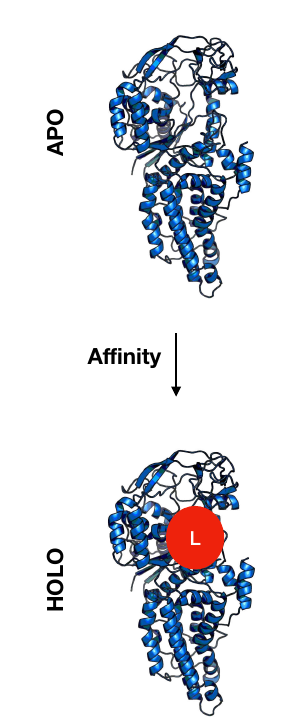
\includegraphics[width=0.7\textwidth]{./img/binding_energy.png}
\end{center}
\end{column}
\end{columns}
\end{frame}

\begin{frame}[label={sec:orgbf87261}]{Designing catalysts: the transition state}
\begin{center}
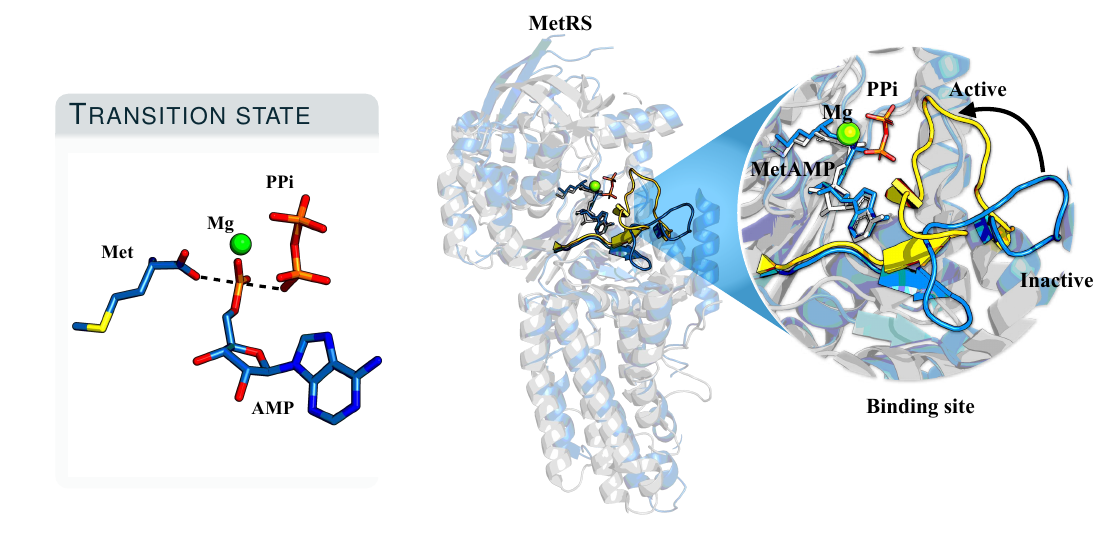
\includegraphics[width=.9\linewidth]{./img/transition_state.png}
\end{center}

\begin{center}
Optimize the binding with the transition state to optimize the catalysis.
\end{center}
\end{frame}

\section*{Benefits and limitations}
\label{sec:orgbca1eae}

\begin{frame}[label={sec:orgafaa3e2}]{Conclusion: Computational Protein Design - A Paradigm Shift}
\begin{block}{Key Takeaways}
\begin{itemize}
\item \alert{\alert{Computational vs. Experimental}}: Computational methods offer speed, precision, and cost-effectiveness, complementing experimental techniques like directed evolution.
\item \alert{\alert{Challenges}}: Navigating vast conformational and sequence spaces, handling computational intensity, and ensuring accurate approximations.
\item \alert{\alert{Applications}}: From designing enzymes for bio-fuels and plastic degradation to predicting protein structures and functions.
\end{itemize}
\end{block}

\begin{block}{Future Directions}
\begin{itemize}
\item \alert{\alert{Integration}}: Combine computational and experimental methods for holistic protein design.
\item \alert{\alert{Technological Advancements}}: Leverage AI and machine learning for enhanced design efficiency.
\end{itemize}
\end{block}
\end{frame}
\end{document}